\documentclass[a0,portrait]{a0poster}

\usepackage{multicol}
\columnsep=100pt

\usepackage[svgnames]{xcolor}
\usepackage{graphicx} 
\usepackage{amsfonts, amsmath, amsthm, amssymb}

\usepackage[font=small,labelfont=bf]{caption}

\usepackage{algorithm} 
\usepackage{algpseudocode}

\newcommand{\fspic}[3][1] {
  \begin{center}\vspace{1cm}
    \includegraphics[width=#1\linewidth]{pics/#2}
    \captionof{figure}{#3}
    \label{#1}
  \end{center}\vspace{1cm}
}

\newcommand {\FlameStream} {FlameStream}

\begin{document}

\begin{minipage}[b]{0.86\linewidth}
  {\huge \textbf{\FlameStream: Model and Runtime for Distributed Stream Processing}}\\
  \bigbreak
  {\large \textbf{Igor E. Kuralenok$^1$, Artem Trofimov$^{1,2}$, Nikita Marshalkin$^{1,2}$, and Boris Novikov$^{1,2}$}}\\
  \bigbreak
  {\large $^1$JetBrains Research, $^2$Saint Petersburg State University}
\end{minipage}
%
\begin{minipage}[b]{0.33\linewidth}
  
\includegraphics[width=10cm]{pics/jetbrains.png} 
\end{minipage}

\vspace{3cm}

\begin{minipage}{.66\linewidth}
  \centering
  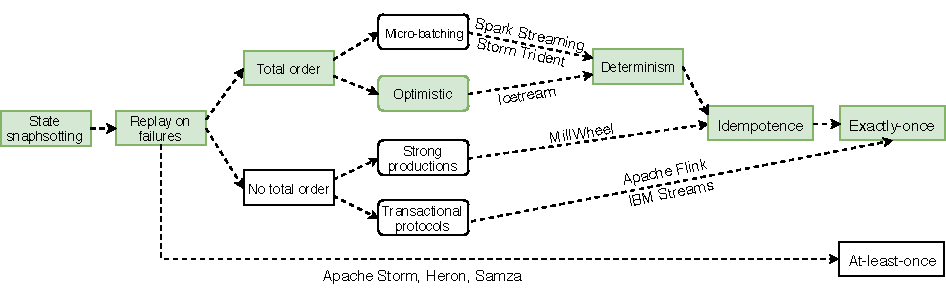
\includegraphics[width=\linewidth]{pics/roadmap}
  \captionof{figure}{The roadmap of approaches for achieving exactly-once and at-least-once guarantees. Green elements indicate the path for our approach}
\end{minipage}

\vspace{3cm}

\begin{multicols}{3} 
  \section*{Graph as a function}
  Determanistic exactly-once processing allows reasoning about execution results as they are determined only by input elements and logical graph.

  \fspic{function}{If computations are determenistic idempotance can be achieved by deduplication buffer at the end of a pipeline}

  \section*{Drifting state}
  Effectively, modern stream processing models allows to work with an operation state in a form of  
  
  \[(in, state) \rightarrow (out, newState)\]
  
  We call this representation a {\em canonical stateful transformation}. Even if models doesn't give such interface, systems provide consistent version through state wrappers. We make such contract explicit by decomposing cycle into two operations: grouping and stateless map

  \fspic{transition}{Any canonical stateful transformation can be expressed by a combination of windowed grouping and stateless map operations}

  \section*{Ordering}
  To manage cyclic flows there is a need to impose strict rules on processing order.

  \fspic{ordering}{Data item with payload $1'$ is the derivative of the item with payload $1$, according to operation $F$. The same is for items with payloads $2'$ and $2$. After merge operation, the order between $1$ and $2$ is preserved. Furthermore, $1'$ follows $1$, and $2'$ follows $2$.}

  \section*{Operations}
  Any stateful pipeline can be expanded into two operations:

  \begin {description}
    \item [Map] applies a user-defined function to the payload of an input item and returns a (possibly empty) sequence of data items with transformed payloads. 
    \item [Grouping] constructs a single item containing a set of consecutive items that have the same value of partition function. The maximum number of items that can be grouped is specified as a parameter  $Window Size.$ 
  \end{description}

  Groupings of different partitions are independent.

  \section*{Optimistic out-of-order processing}
  Only grouping results depends on order elements as it is the only operation that maintains state (partial widows). 
  
  It has a well-defined state structure that allows to effectively provide correct results.

  It optimistically produces tuples as they were in-order. I case of reordering it is locally generates correct tuples and sends tombstones for incorrect ones. 
  \fspic{grouping-invalidation}{On arrival of out-of-order item, it is inserted in the correct location of the correcponding bucket. Valid elements containing new item are produced, and invalid ones are invalidated by sending a tombstone for it down the stream}

  \section*{Garbage filtering}
  In case of reordering invalid tuples are generated. In order to return only correct tuples to users there is a barrier at the end of the pipeline. It passes correct items and filters out incorrect ones.

  \fspic{happy-man}{Barrier collects elements in a buffer and removes item for which tombstones have arrived. Periodically it flushes buffer and returnes elements to the end-user. Punctuations used in OOP approach can be used as flush-trigger}

  \section*{Consistency}
  Model properties allows us to provide strong guarantees on processing results - exaclty-once semantics.

  Total order and determinism allows us to filter out duplicates at the barrier by simply comparing elements timestamps with last evicted item.

  Moreover state structures enables performing asynchronous snapshot of operations' states.

  \fspic[.7]{bucket-parts}{Grouping buckets can be divided into two parts: immutable and mutable. The separator is the time of the last received punction (we call it minimal time). State snapshot for any time before minimal time can be obtained by extracting window-sized sublist}
\end{multicols}

\vspace{3cm}

\begin{minipage}{\linewidth}
  \fspic[.5]{comparison}{Comparison}
\end{minipage}
\end{document}
